\chapter{Química del estado sólido: bandas, defectos y semiconductores}\label{ch:b3:solid-state}

Un panel solar en un tejado y el diodo emisor de luz de una lámpara están hechos del
mismo tipo de cristal, silicio o un compuesto de galio con nitrógeno, arsénico
o fósforo, en el que se han introducido a propósito unos pocos átomos de impurezas por millón.
Su funcionamiento lo fijan dos cosas que una molécula no tiene: bandas de
niveles de energía, con una \omterm{def:b3:solid-state:band}{banda prohibida} cuya anchura determina qué luz absorbe o
emite un cristal, y defectos, que transportan las cargas. Este capítulo construye las bandas
a partir de los orbitales moleculares, cuenta los portadores de un \omterm{def:b3:solid-state:classes}{semiconductor} y trata
los átomos ausentes o mal situados como especies químicas con sus propios equilibrios,
hasta el \omterm{def:b3:solid-state:ionic-conductor}{electrolito sólido} de la sonda de oxígeno del escape de un coche.

\begin{recall}
El volumen del primer año definió los cristales, el enlace metálico, los cristales iónicos y
covalentes, los sitios intersticiales y las aleaciones, y la ecuación de Nernst; el volumen
del segundo año, el método de Hückel y la integral de resonancia $\beta$.
El \cref{ch:b3:x-ray-diffraction} dio la \omterm{def:b3:x-ray-diffraction:reciprocal}{red recíproca}, y
el \cref{ch:b3:partition-functions}, la \omterm{def:b3:partition-functions:boltzmann}{distribución de Boltzmann} y la
\omterm{def:b3:partition-functions:statistical-entropy}{entropía estadística} $S = k\ln W$.
\end{recall}

\begin{omfigure}
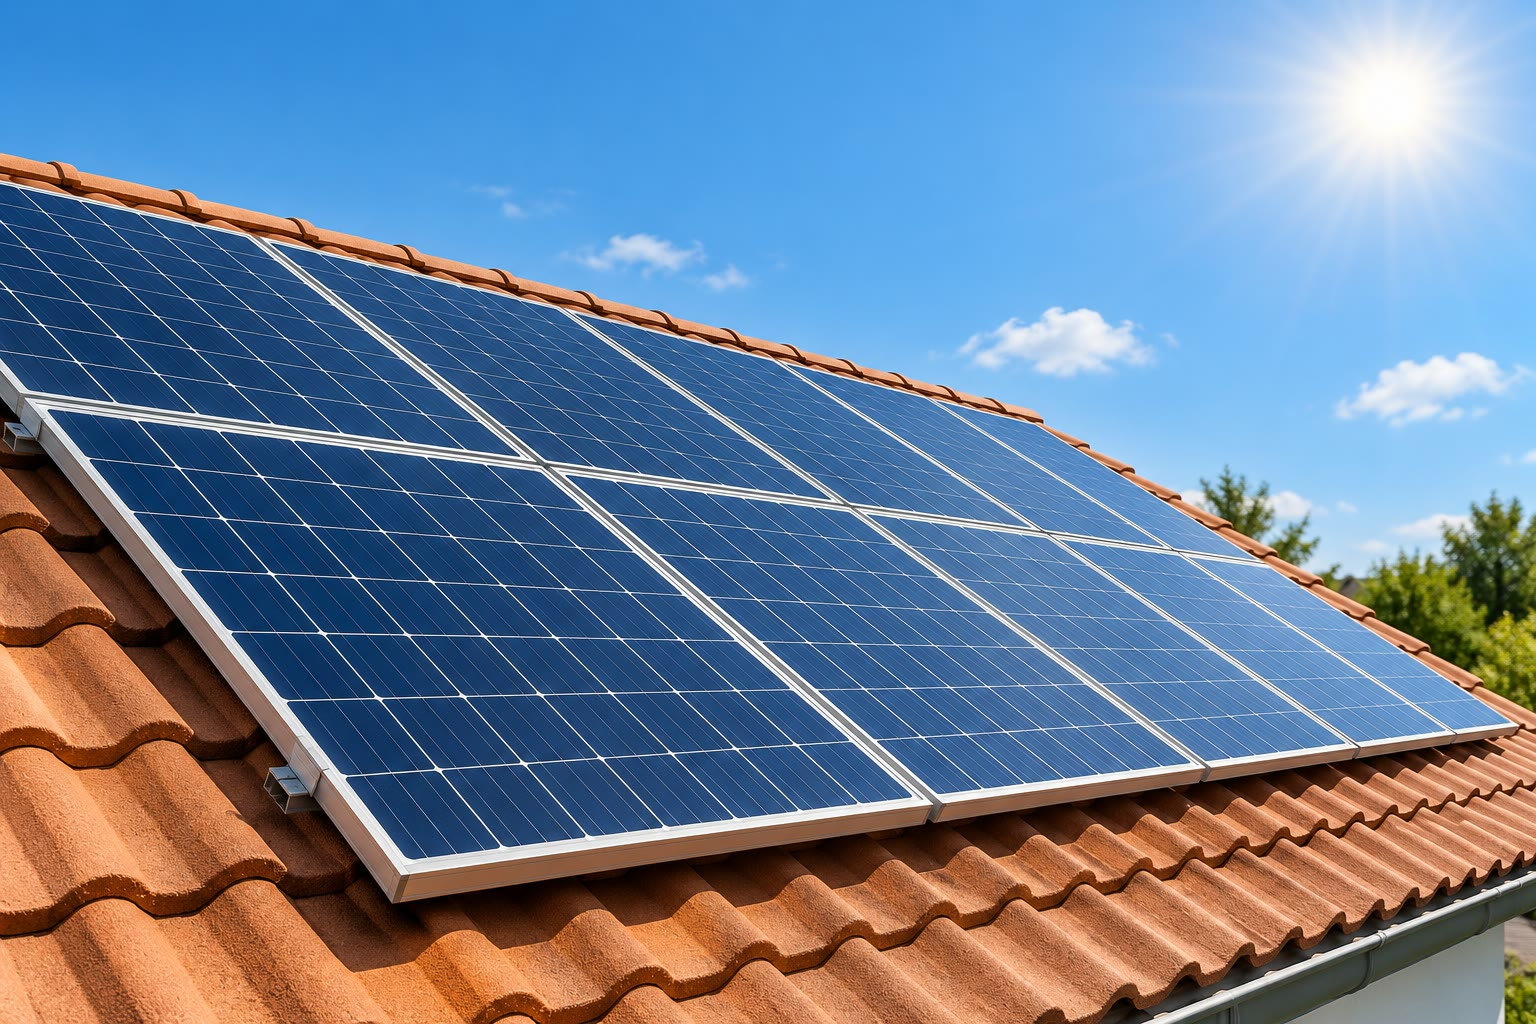
\includegraphics[width=0.6\linewidth]{images/book4/ai/b3-22-solar-panels.jpg}

{\small Paneles solares sobre un tejado de tejas: cada célula es una fina lámina de silicio en
la que la luz eleva electrones a través de una \omterm{def:b3:solid-state:band}{banda prohibida} de alrededor de un electronvoltio.}
\end{omfigure}

\section{De los orbitales a las bandas}

Considérese una cadena de $N$ átomos idénticos, cada uno con un orbital s, en la aproximación
de Hückel: integral de Coulomb $\alpha$ en cada átomo, integral de resonancia $\beta < 0$
entre vecinos y cero en los demás casos.

\begin{theorem}[Niveles de una cadena de Hückel]\label{thm:b3:solid-state:chain}
Los $N$ orbitales moleculares de una cadena lineal de $N$ átomos tienen las energías
\[
  E_k = \alpha + 2\beta\cos\frac{k\pi}{N + 1}, \qquad k = 1, \dots, N,
\]
con coeficientes $c_j^{(k)} \propto \sin\bigl(jk\pi/(N + 1)\bigr)$ en el átomo $j$. Cuando $N \to \infty$, los niveles llenan densamente el
intervalo de $\alpha + 2\beta$ a $\alpha - 2\beta$: una banda de anchura $4|\beta|$.
\end{theorem}

\begin{proof}
Las ecuaciones seculares son $\beta c_{j-1} + (\alpha - E)c_j + \beta c_{j+1} = 0$ para $j = 1, \dots, N$, con $c_0 = c_{N+1} = 0$
(no hay átomo allí). Pruébese $c_j = \sin(j\theta)$: como $\sin((j - 1)\theta) + \sin((j + 1)\theta) = 2\cos\theta\sin(j\theta)$, cada
ecuación se convierte en $(\alpha - E + 2\beta\cos\theta)\sin(j\theta) = 0$, luego $E = \alpha + 2\beta\cos\theta$. La condición $c_0 = 0$ se cumple
para todo $\theta$, y $c_{N+1} = \sin((N + 1)\theta) = 0$ exige $\theta = k\pi/(N + 1)$; $k = 1, \dots, N$ da $N$ niveles
distintos (los demás los repiten o se anulan). El más bajo y el más alto son
$\alpha \pm 2\beta\cos(\pi/(N + 1))$, que tienden a $\alpha \pm 2\beta$; la separación entre vecinos es como máximo
$2|\beta|\pi/(N + 1)$, que tiende a cero.
\end{proof}

Para $N = 2$, el teorema da $\alpha \pm \beta$, los orbitales del sistema $\pi$ del eteno; para
$N = 6$, el hexatrieno de cadena abierta. En tres dimensiones ocurre lo mismo con
todo tipo de orbital atómico: los orbitales s dan una banda s, los orbitales p una banda p,
y cada banda admite $2N$ electrones para $N$ átomos.

\begin{definition}[Bandas]\label{def:b3:solid-state:band}
Una \emph{banda de energía}\index{banda de energia@banda de energía} de un cristal es un intervalo continuo de
energías monoelectrónicas permitidas, formado a partir de los orbitales de todos sus átomos. Una
\emph{banda prohibida}\index{banda prohibida} $E_g$ es un intervalo de energías sin niveles entre dos
bandas. En un \omterm{def:b3:solid-state:classes}{semiconductor} o en un \omterm{def:b3:solid-state:classes}{aislante} a temperatura cero, la banda llena
más alta es la \emph{banda de valencia}\index{banda de valencia}, y la banda vacía más baja,
la \emph{banda de conducción}\index{banda de conduccion@banda de conducción}.
\end{definition}

\begin{definition}[Densidad de estados y nivel de Fermi]\label{def:b3:solid-state:fermi}
La \emph{densidad de estados}\index{densidad de estados} $g(E)$ es el número de
niveles por unidad de energía (y por átomo o por unidad de volumen) en torno a la energía $E$.
El \emph{nivel de Fermi}\index{nivel de Fermi} $E_F$ es la energía a la que un nivel tiene
una probabilidad $1/2$ de estar ocupado; a temperatura cero, todos los niveles por debajo de él están
llenos y todos los de encima, vacíos.
\end{definition}

\begin{omfigure}
\begin{tikzpicture}
\begin{axis}[width=0.78\linewidth, height=6.2cm, xmin=0.3, xmax=7.6, ymin=-2.3, ymax=2.3,
  axis lines=left, xtick={1,2,3,4,5,6.6}, xticklabels={2,4,8,16,64,$\infty$: $g(E)$},
  xlabel={número de átomos $N$}, ylabel={$(E - \alpha)/|\beta|$},
  ytick={-2,-1,0,1,2}, tick label style={font=\small}, label style={font=\small}]
\addplot[only marks, mark=-, mark size=7pt, omDef, thick] table[x=col, y=e] {figdata/out/bachelor-3-band-chain.dat};
\addplot[omThm, thick] table[x expr=6.0+0.55*\thisrow{g}, y=e] {figdata/out/bachelor-3-band-chain-b.dat};
\draw[black!40, dashed] (axis cs:0.3,-2) -- (axis cs:7.6,-2);
\draw[black!40, dashed] (axis cs:0.3,2) -- (axis cs:7.6,2);
\draw[<->, black!60] (axis cs:5.6,-2) -- (axis cs:5.6,2) node[midway, left, font=\scriptsize] {$4|\beta|$};
\end{axis}
\end{tikzpicture}

{\small Niveles de Hückel de cadenas de 2 a 64 átomos (una línea corta por nivel;
con $\beta < 0$, los niveles enlazantes están abajo). Los niveles se apiñan en una banda
entre $\alpha + 2\beta$ y $\alpha - 2\beta$; a la derecha, la \omterm{def:b3:solid-state:fermi}{densidad de estados} de la cadena
infinita, máxima en los bordes de la banda.}
\end{omfigure}

\begin{proposition}[Llenado de las bandas]\label{prop:b3:solid-state:filling}
Un cristal cuya banda ocupada más alta está parcialmente llena conduce la electricidad
como un metal; un cristal cuyas bandas están llenas o vacías, con una \omterm{def:b3:solid-state:band}{banda prohibida}
entre ellas, no conduce a temperatura cero.
\end{proposition}

\begin{proof}[Argumento]
En un campo eléctrico, los electrones ganan un poco de energía y de momento lineal: deben
pasar a niveles vacíos justo por encima de los que ocupan. En una banda parcialmente
llena, esos niveles están inmediatamente por encima del \omterm{def:b3:solid-state:fermi}{nivel de Fermi}, sin coste energético. En
una banda llena, todos los niveles están ocupados y el siguiente vacío está al otro lado de la \omterm{def:b3:solid-state:band}{banda prohibida};
además, una banda llena no transporta corriente neta, ya que por cada electrón que se mueve
en un sentido otro se mueve en el sentido opuesto.
\end{proof}

El sodio, con un electrón 3s por átomo, llena a medias su banda s: es un metal.
El magnesio, con dos, llenaría exactamente su banda s, pero las bandas s y p
se solapan, de modo que también es un metal. El diamante y el silicio tienen cuatro electrones de valencia
por átomo en orbitales que se desdoblan en una banda enlazante llena y una banda
antienlazante vacía, separadas por una \omterm{def:b3:solid-state:band}{banda prohibida}.

\begin{definition}[Semiconductores y aislantes]\label{def:b3:solid-state:classes}
Un \emph{semiconductor}\index{semiconductor} es un sólido con una \omterm{def:b3:solid-state:band}{banda prohibida} lo bastante
estrecha (hasta unos \qty{3}{eV}) para que un número medible de electrones la atraviese
a temperatura ordinaria o tras el dopado; un \emph{aislante}\index{aislante}
tiene una \omterm{def:b3:solid-state:band}{banda prohibida} tan ancha que no conduce.
\end{definition}

\begin{omfigure}
\begin{tikzpicture}[font=\small]
  \foreach \x/\name in {0/metal, 3.6/semiconductor, 7.2/aislante} {
    \node[font=\small\bfseries] at (\x+0.8,4.3) {\name};
  }
  % metal: one partly filled band
  \fill[omDef!55] (0,0.4) rectangle (1.6,2.0);
  \draw (0,0.4) rectangle (1.6,3.4);
  \draw[omThm, thick] (-0.25,2.0) -- (1.85,2.0) node[right, font=\scriptsize] {$E_F$};
  % semiconductor: small gap
  \fill[omDef!55] (3.6,0.4) rectangle (5.2,1.7);
  \draw (3.6,0.4) rectangle (5.2,1.7);
  \draw (3.6,2.5) rectangle (5.2,3.8);
  \draw[omThm, thick] (3.35,2.1) -- (5.45,2.1) node[right, font=\scriptsize] {$E_F$};
  \draw[<->] (4.4,1.7) -- (4.4,2.5) node[pos=0.8, right, font=\scriptsize] {$E_g$};
  % insulator: large gap
  \fill[omDef!55] (7.2,0.4) rectangle (8.8,1.2);
  \draw (7.2,0.4) rectangle (8.8,1.2);
  \draw (7.2,3.2) rectangle (8.8,4.0);
  \draw[omThm, thick] (6.95,2.2) -- (9.05,2.2) node[right, font=\scriptsize] {$E_F$};
  \draw[<->] (8.0,1.2) -- (8.0,3.2) node[pos=0.75, right, font=\scriptsize] {$E_g$};
  \node[font=\scriptsize, anchor=east] at (3.5,1.05) {valencia};
  \node[font=\scriptsize, anchor=east] at (3.5,3.15) {conducción};
  \draw[->] (-0.6,0.2) -- (-0.6,3.9) node[above, font=\scriptsize] {$E$};
\end{tikzpicture}

{\small Llenado de las bandas a temperatura cero (niveles llenos sombreados). Un metal tiene una
banda parcialmente llena y su \omterm{def:b3:solid-state:fermi}{nivel de Fermi} dentro de ella; un \omterm{def:b3:solid-state:classes}{semiconductor} y un
\omterm{def:b3:solid-state:classes}{aislante} tienen una \omterm{def:b3:solid-state:band}{banda de valencia} llena y una \omterm{def:b3:solid-state:band}{banda de conducción} vacía, con el \omterm{def:b3:solid-state:fermi}{nivel
de Fermi} en la \omterm{def:b3:solid-state:band}{banda prohibida}, estrecha en el primero y ancha en el segundo.}
\end{omfigure}

\section{Semiconductores}

\begin{definition}[Portadores]\label{def:b3:solid-state:carriers}
Un \emph{semiconductor intrínseco}\index{semiconductor intrinseco@semiconductor intrínseco} es un \omterm{def:b3:solid-state:classes}{semiconductor}
puro, cuyos portadores proceden todos de electrones excitados a través de la \omterm{def:b3:solid-state:band}{banda prohibida}. Un
\emph{portador de carga}\index{portador de carga} es una partícula móvil que transporta
corriente: un electrón de la \omterm{def:b3:solid-state:band}{banda de conducción}, o un \emph{hueco}\index{hueco}, un
nivel vacío de la \omterm{def:b3:solid-state:band}{banda de valencia}, que se mueve como una carga positiva.
\end{definition}

\begin{theorem}[Concentración intrínseca de portadores]\label{thm:b3:solid-state:intrinsic}
Con $N_c$ y $N_v$, las densidades efectivas de estados de las \omterm{def:b3:solid-state:band}{bandas de conducción} y de
valencia (se admiten), las concentraciones de electrones y de \omterm{def:b3:solid-state:carriers}{huecos} de un \omterm{def:b3:solid-state:classes}{semiconductor}
cuyo \omterm{def:b3:solid-state:fermi}{nivel de Fermi} está a más de unos pocos $kT$ de ambos bordes de banda son
\[
  n = N_c\,\eu^{-(E_c - E_F)/kT}, \qquad p = N_v\,\eu^{-(E_F - E_v)/kT},
\]
y, en un \omterm{def:b3:solid-state:carriers}{semiconductor intrínseco},
\[
  n = p = n_i = \sqrt{N_cN_v}\,\eu^{-E_g/2kT}.
\]
\end{theorem}

\begin{proof}
La ocupación de un nivel de energía $E$ es $f(E) = 1/(1 + \eu^{(E - E_F)/kT})$. Cuando
$E - E_F \gg kT$, $f \approx \eu^{-(E - E_F)/kT}$, una cola de Boltzmann. Sumándola sobre los niveles de la \omterm{def:b3:solid-state:band}{banda de
conducción}, $n = \int g_c(E)\eu^{-(E - E_F)/kT}\,\dd E = \eu^{-(E_c - E_F)/kT}\int g_c(E)\eu^{-(E - E_c)/kT}\,\dd E$, y la última integral es por
definición $N_c$. Los \omterm{def:b3:solid-state:carriers}{huecos} son niveles vacíos, con probabilidad $1 - f \approx \eu^{-(E_F - E)/kT}$ en la
\omterm{def:b3:solid-state:band}{banda de valencia}; los mismos pasos dan $p$. Entonces $np = N_cN_v\eu^{-(E_c - E_v)/kT} = N_cN_v\eu^{-E_g/kT}$, y en un cristal puro
cada electrón excitado deja un \omterm{def:b3:solid-state:carriers}{hueco}: $n = p$, luego $n = \sqrt{np}$.
\end{proof}

\begin{proposition}[Ley de acción de masas]\label{prop:b3:solid-state:mass-action}
En todo \omterm{def:b3:solid-state:classes}{semiconductor} en equilibrio, dopado o no, $np = n_i^2$.
\end{proposition}

\begin{proof}
El producto $np = N_cN_v\eu^{-E_g/kT}$ hallado en la demostración del
\cref{thm:b3:solid-state:intrinsic} no contiene $E_F$: es el mismo sea lo que sea lo que
fije el \omterm{def:b3:solid-state:fermi}{nivel de Fermi}, e igual a su valor intrínseco $n_i^2$. Es la
constante de equilibrio de $\text{nada} \rightleftharpoons \mathrm e^- + \mathrm h^+$, como el producto iónico del agua.
\end{proof}

\begin{omfigure}
% ledger: eg:Si.E0, eg:Si.a, eg:Si.b, eg:Ge.E0, eg:Ge.a, eg:Ge.b, dos:Si.Nc, dos:Si.Nv, dos:Ge.Nc, dos:Ge.Nv, dop:Si.P
\begin{tikzpicture}
\begin{axis}[name=a, width=0.45\linewidth, height=5.6cm, xmin=1.2, xmax=4.2, ymin=4, ymax=18,
  axis lines=left, xlabel={$1000\,\mathrm K/T$}, ylabel={$\log_{10}(n_i/\unit{cm^{-3}})$},
  tick label style={font=\scriptsize}, label style={font=\small}]
\addplot[omDef, thick] table[x=invT, y=lgSi] {figdata/out/bachelor-3-semiconductor-carriers.dat};
\addplot[omThm, thick] table[x=invT, y=lgGe] {figdata/out/bachelor-3-semiconductor-carriers.dat};
\node[font=\scriptsize, omDef] at (axis cs:3.4,8.3) {Si};
\node[font=\scriptsize, omThm, anchor=south west] at (axis cs:3.4,14.0) {Ge};
\end{axis}
\begin{axis}[at={(a.east)}, anchor=west, xshift=1.7cm, width=0.45\linewidth, height=5.6cm,
  xmin=1, xmax=25, ymin=10, ymax=17, axis lines=left,
  xlabel={$1000\,\mathrm K/T$}, ylabel={$\log_{10}(n/\unit{cm^{-3}})$},
  tick label style={font=\scriptsize}, label style={font=\small}]
\addplot[omDef, thick] table[x=invT, y=lgn] {figdata/out/bachelor-3-semiconductor-carriers-b.dat};
\addplot[black!45, dashed, unbounded coords=jump, restrict y to domain=10:17] table[x=invT, y=lgni] {figdata/out/bachelor-3-semiconductor-carriers-b.dat};
\node[font=\scriptsize, anchor=west] at (axis cs:2.6,16.4) {intrínseco};
\node[font=\scriptsize] at (axis cs:12,15.35) {saturación, $n = N_D$};
\node[font=\scriptsize] at (axis cs:20,13.2) {congelación};
\end{axis}
\end{tikzpicture}

{\small Izquierda: concentraciones intrínsecas de portadores del silicio y del germanio en función de
$1/T$ (modelo con las \omterm{def:b3:solid-state:band}{bandas prohibidas} y las densidades efectivas de estados medidas); las
pendientes son próximas a $-E_g/2k$. Derecha: electrones en silicio dopado con
$\qty{1e15}{cm^{-3}}$ de fósforo: a baja temperatura, los donadores retienen sus electrones
(congelación); de unos 150 a \qty{500}{K}, todos están ionizados ($n = N_D$), y a alta
temperatura dominan los portadores intrínsecos (trazo discontinuo, $n_i$).}
\end{omfigure}

\begin{definition}[Bandas prohibidas directas e indirectas]\label{def:b3:solid-state:gap-types}
Un \omterm{def:b3:solid-state:classes}{semiconductor} tiene una \emph{banda prohibida directa}\index{banda prohibida directa} cuando la
cima de su \omterm{def:b3:solid-state:band}{banda de valencia} y el fondo de su \omterm{def:b3:solid-state:band}{banda de conducción} se dan con el mismo
momento lineal del electrón, de modo que un fotón por sí solo puede llevar un electrón al otro lado, y una
\emph{banda prohibida indirecta}\index{banda prohibida indirecta} cuando no es así, de modo que la
transición necesita además una vibración de la red.
\end{definition}

% ledger: eg:Si, eg:Ge, eg:GaAs, eg:GaN, eg:GaP
El silicio (\qty{1.12}{eV}) y el germanio (\qty{0.66}{eV}) tienen \omterm{def:b3:solid-state:gap-types}{bandas prohibidas indirectas}:
absorben la luz lo bastante bien en una capa gruesa, lo que conviene a una célula solar, pero
la emiten muy mal. El arseniuro de galio (\qty{1.42}{eV}) y el nitruro de galio (unos
\qty{3.4}{eV}) tienen \omterm{def:b3:solid-state:gap-types}{bandas prohibidas directas}, la base de los diodos emisores de luz infrarroja y
azul y de los láseres; el fosfuro de galio (\qty{2.26}{eV}) es indirecto, pero emite luz verde
cuando está dopado. El color de muchos pigmentos también se debe a una \omterm{def:b3:solid-state:band}{banda prohibida}: un cristal
absorbe todos los fotones con $h\nu > E_g$, de modo que el sulfuro de cadmio, con una \omterm{def:b3:solid-state:band}{banda prohibida} en el azul,
es amarillo.

\begin{definition}[Dopado]\label{def:b3:solid-state:doping}
Un \emph{dopante}\index{dopante} es un átomo extraño introducido a propósito en un \omterm{def:b3:solid-state:classes}{semiconductor},
en pequeñas cantidades, para aportar portadores. En un \emph{semiconductor de
tipo n}\index{semiconductor de tipo n}, el dopante tiene un electrón de valencia más
que el átomo al que sustituye (fósforo en silicio) y lo cede a la
\omterm{def:b3:solid-state:band}{banda de conducción} desde un \emph{nivel donador}\index{nivel donador} situado justo por debajo de esa
banda; en un \emph{semiconductor de tipo p}\index{semiconductor de tipo p}, tiene uno
menos (boro en silicio) y acepta un electrón de la \omterm{def:b3:solid-state:band}{banda de valencia} en un
\emph{nivel aceptor}\index{nivel aceptor} situado justo por encima de ella, dejando un \omterm{def:b3:solid-state:carriers}{hueco}.
\end{definition}

\begin{omfigure}
\begin{tikzpicture}[font=\small]
  \foreach \x in {0, 5.2} {
    \fill[omDef!35] (\x,0) rectangle (\x+3.6,1.0);
    \fill[omDef!12] (\x,2.6) rectangle (\x+3.6,3.6);
    \node[font=\scriptsize] at (\x+1.8,0.5) {valencia};
    \node[font=\scriptsize] at (\x+1.8,3.1) {conducción};
  }
  \foreach \i in {0,...,5} { \draw[omThm, thick] (0.25+\i*0.55,2.35) -- (0.6+\i*0.55,2.35); }
  \node[font=\scriptsize, anchor=west] at (0.1,1.95) {niveles donadores, \qty{0.045}{eV} por debajo};
  \draw[->, omThm] (0.42,2.42) -- (0.42,2.9);
  \fill[omThm] (0.42,2.95) circle (1.6pt);
  \foreach \i in {0,...,5} { \draw[omMeth, thick] (5.45+\i*0.55,1.25) -- (5.8+\i*0.55,1.25); }
  \node[font=\scriptsize, anchor=west] at (5.3,1.6) {niveles aceptores, \qty{0.045}{eV} por encima};
  \draw[->, omMeth] (5.62,0.7) -- (5.62,1.18);
  \draw[omMeth, fill=white] (5.62,0.62) circle (1.8pt);
  \node[font=\small\bfseries] at (1.8,4.0) {tipo n: P en Si};
  \node[font=\small\bfseries] at (7.0,4.0) {tipo p: B en Si};
\end{tikzpicture}

{\small \omterm{def:b3:solid-state:doping}{Niveles donadores} y aceptores en la \omterm{def:b3:solid-state:band}{banda prohibida} del silicio (\omterm{def:b3:solid-state:band}{banda prohibida} no a escala: los
niveles de los \omterm{def:b3:solid-state:doping}{dopantes} están a unos 0.045 eV de los bordes de las bandas, y la \omterm{def:b3:solid-state:band}{banda prohibida} mide 1.12 eV). Un
donador cede su electrón (punto) a la \omterm{def:b3:solid-state:band}{banda de conducción}; un aceptor toma uno
de la \omterm{def:b3:solid-state:band}{banda de valencia} y deja un \omterm{def:b3:solid-state:carriers}{hueco} (círculo).}
\end{omfigure}

% ledger: dop:Si.P, dop:Si.B
El \omterm{def:b3:solid-state:doping}{nivel donador} del fósforo está \qty{0.045}{eV} por debajo de la \omterm{def:b3:solid-state:band}{banda de conducción} del
silicio, menos de $2kT$ a temperatura ambiente, y el \omterm{def:b3:solid-state:doping}{nivel aceptor} del boro, otro tanto
por encima de la \omterm{def:b3:solid-state:band}{banda de valencia}: a \qty{300}{K}, casi todos los \omterm{def:b3:solid-state:doping}{dopantes} están ionizados. Por eso
un átomo de \omterm{def:b3:solid-state:doping}{dopante} por cada $10^7$ átomos de silicio ($\qty{5e15}{cm^{-3}}$) multiplica la
concentración de electrones por unos cientos de miles.

\begin{method}[Portadores de un semiconductor dopado]\label{met:b3:solid-state:doping}
\begin{enumerate}
  \item Comprobar que la temperatura está en el intervalo de saturación (\omterm{def:b3:solid-state:doping}{dopantes} totalmente
        ionizados, $N_D \gg n_i$): entonces los portadores mayoritarios son $n \approx N_D$ (o $p \approx N_A$).
  \item Obtener los portadores minoritarios a partir de la ley de acción de masas: $p = n_i^2/N_D$.
  \item Situar el \omterm{def:b3:solid-state:fermi}{nivel de Fermi}: $E_c - E_F = kT\ln(N_c/n)$ o, respecto del nivel intrínseco,
        $E_F - E_i = kT\ln(n/n_i)$.
  \item Si hay presentes \omterm{def:b3:solid-state:doping}{dopantes} de ambos tipos, usar la diferencia $N_D - N_A$.
\end{enumerate}
\end{method}

\begin{definition}[Unión p--n]\label{def:b3:solid-state:junction}
Una \emph{unión p--n}\index{union p--n@unión p--n} es la frontera, dentro de un mismo cristal,
entre una región de tipo p y una de tipo n.
\end{definition}

En una \omterm{def:b3:solid-state:junction}{unión p--n}, los electrones difunden del lado n al lado p y los \omterm{def:b3:solid-state:carriers}{huecos}
en sentido contrario, dejando una capa delgada vaciada de portadores en la que los \omterm{def:b3:solid-state:doping}{dopantes}
ionizados fijos crean un campo eléctrico; en el equilibrio, el \omterm{def:b3:solid-state:fermi}{nivel de Fermi} es el
mismo a ambos lados. Una tensión aplicada en un sentido rebaja la barrera y circula la
corriente; en el otro sentido la eleva: es un diodo. En un diodo emisor de luz, los electrones
y los \omterm{def:b3:solid-state:carriers}{huecos} inyectados a través de la unión se recombinan y emiten fotones de energía
próxima a $E_g$; en una célula solar, los fotones absorbidos cerca de la unión crean
pares electrón--hueco que el campo separa, y circula una corriente por el
circuito exterior.

\begin{omfigure}
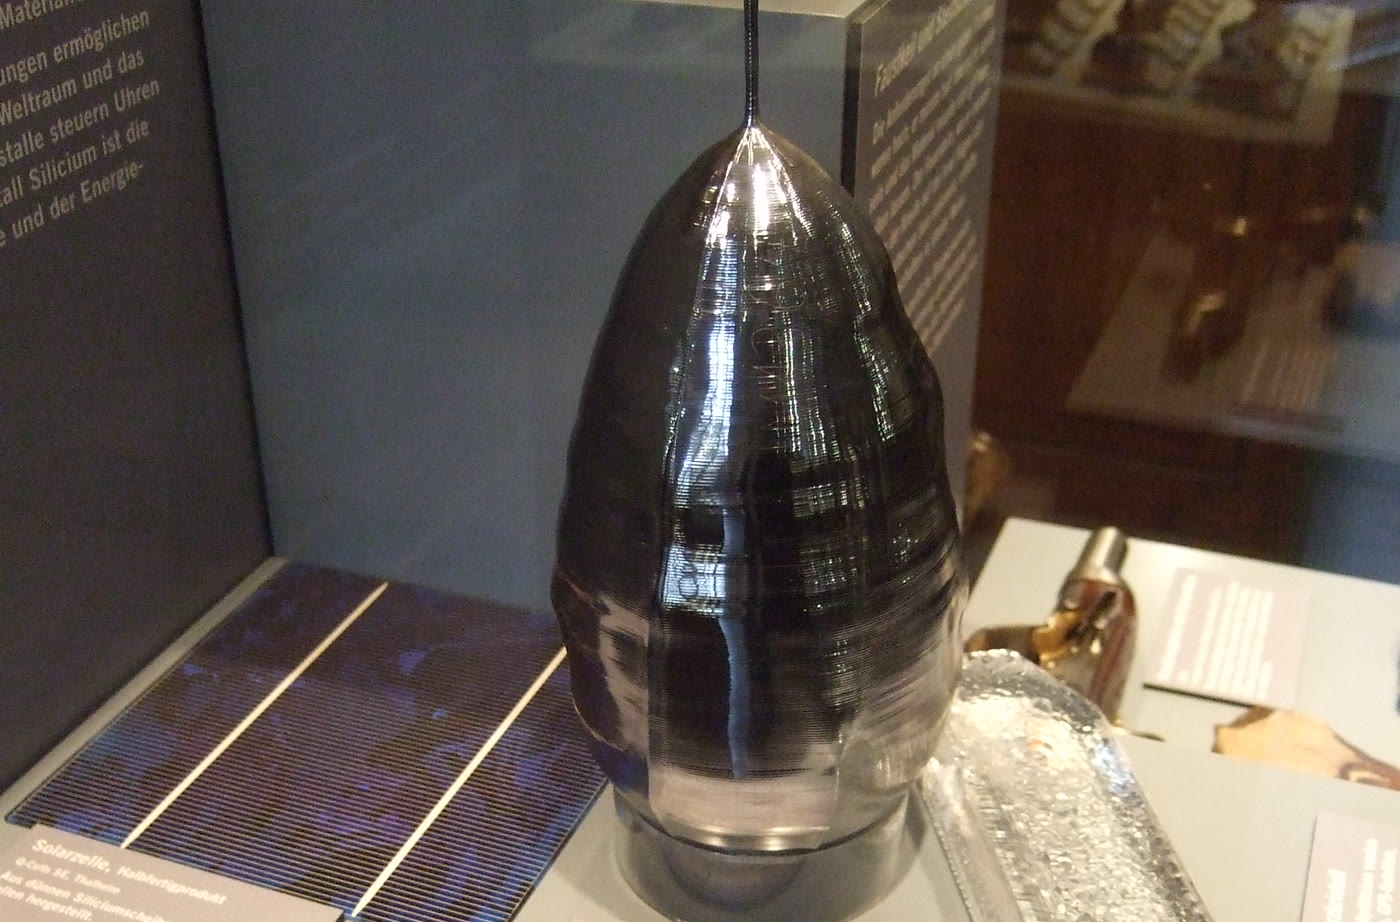
\includegraphics[width=0.5\linewidth]{images/book4/silicon-boule.jpg}

{\small Un monocristal de silicio extraído del fundido, junto a una célula
solar hecha con una lámina de un cristal así. Fotografía: Sebastian Wallroth,
dominio público.}
\end{omfigure}

\begin{inthelab}[Crecimiento de un cristal de silicio]
En el método de Czochralski, se funde silicio policristalino muy puro en un
crisol de sílice bajo argón, a una temperatura algo superior a su punto de fusión, con el
\omterm{def:b3:solid-state:doping}{dopante} añadido al fundido. Un pequeño cristal semilla, montado en una varilla giratoria, se sumerge en
el fundido y se eleva lentamente: el silicio cristaliza sobre él con la
orientación de la semilla, y la velocidad de extracción y de rotación fija el diámetro. El lingote
se sierra después en obleas de menos de un milímetro de espesor. El silano y los gases
\omterm{def:b3:solid-state:doping}{dopantes} fosfina y arsina, usados en etapas posteriores, son pirofóricos o muy tóxicos,
y solo se manipulan en sistemas industriales estancos.
\end{inthelab}

\section{Defectos puntuales}

\begin{definition}[Defectos puntuales]\label{def:b3:solid-state:defects}
Un \emph{defecto puntual}\index{defecto puntual} es una desviación respecto del cristal
perfecto localizada en una posición: una vacante, un átomo intersticial o un átomo
extraño. En un cristal iónico, un \emph{defecto de Schottky}\index{defecto de Schottky} es un
par de vacantes, una catiónica y una aniónica, cuyos iones se han ido a la
superficie; un \emph{defecto de Frenkel}\index{defecto de Frenkel} es un par formado por una
vacante y el ion que la dejó, situado en una posición intersticial.
\end{definition}

\begin{omfigure}
\begin{tikzpicture}[scale=0.62]
  \begin{scope}
  \foreach \i in {0,...,5} \foreach \j in {0,...,4} {
    \pgfmathtruncatemacro{\pty}{mod(\i+\j,2)}
    \ifnum\pty=0 \fill[omDef!70] (\i,\j) circle (0.2); \else \fill[omThm!25] (\i,\j) circle (0.38); \draw[omThm!60] (\i,\j) circle (0.38); \fi
  }
  \fill[white] (2,2) circle (0.45); \draw[dashed] (2,2) circle (0.3);
  \fill[white] (3,2) circle (0.45); \draw[dashed] (3,2) circle (0.38);
  \node[font=\small\bfseries] at (2.5,5.0) {Schottky (NaCl)};
  \end{scope}
  \begin{scope}[xshift=8cm]
  \foreach \i in {0,...,5} \foreach \j in {0,...,4} {
    \pgfmathtruncatemacro{\pty}{mod(\i+\j,2)}
    \ifnum\pty=0 \fill[black!45] (\i,\j) circle (0.2); \else \fill[omMeth!25] (\i,\j) circle (0.38); \draw[omMeth!60] (\i,\j) circle (0.38); \fi
  }
  \fill[white] (2,2) circle (0.3); \draw[dashed] (2,2) circle (0.22);
  \fill[black!45] (2.5,2.5) circle (0.2);
  \draw[->, thick] (2.1,2.1) -- (2.38,2.38);
  \node[font=\small\bfseries] at (2.5,5.0) {Frenkel (AgCl)};
  \end{scope}
\end{tikzpicture}

{\small \omterm{def:b3:solid-state:defects}{Defectos puntuales} en una capa de un cristal de tipo sal gema (puntos pequeños: cationes;
círculos grandes: aniones; trazo discontinuo: vacantes). Izquierda: un par de Schottky, en el que faltan un catión
y un anión. Derecha: un par de Frenkel, un ion plata desplazado de su posición
a una posición intersticial.}
\end{omfigure}

\begin{theorem}[Concentración de equilibrio de los defectos de Schottky]\label{thm:b3:solid-state:schottky}
En un cristal MX de $N$ unidades fórmula, el número $n$ de pares de Schottky en el
equilibrio, con una entalpía de formación $\Delta H_S$ por par y $n \ll N$, es
\[
  \frac{n}{N} = \eu^{-\Delta H_S/2kT}.
\]
\end{theorem}

\begin{proof}
Crear $n$ pares cuesta $n\,\Delta H_S$ y aporta una entropía configuracional, procedente de las
$\binom{N}{n}$ maneras de elegir las vacantes catiónicas y otras tantas para las aniónicas:
$S = 2k\ln\frac{N!}{n!(N - n)!}$. Con la fórmula de Stirling, $\ln x! \approx x\ln x - x$,
\[
  G(n) = n\,\Delta H_S - 2kT\bigl[N\ln N - n\ln n - (N - n)\ln(N - n)\bigr].
\]
En el equilibrio, $\dd G/\dd n = 0$: $\Delta H_S - 2kT\ln\frac{N - n}{n} = 0$, luego $n/(N - n) = \eu^{-\Delta H_S/2kT}$, y $n/N$ para
$n \ll N$. La entropía vibracional de los defectos, despreciada aquí, multiplica el
resultado por un factor constante.
\end{proof}

\begin{proposition}[Defectos de Frenkel]\label{prop:b3:solid-state:frenkel}
Con $N$ iones de la especie móvil, $N_i$ posiciones intersticiales disponibles para ellos y
$\Delta H_F$ la entalpía de formación de un par, el número de pares de Frenkel es $n =
\sqrt{NN_i}\,\eu^{-\Delta H_F/2kT}$ (para $n \ll N, N_i$).
\end{proposition}

\begin{proof}
Ahora la entropía es $S = k\ln\binom{N}{n} + k\ln\binom{N_i}{n}$, y la misma minimización da
\[
  \Delta H_F = kT\ln\frac{(N - n)(N_i - n)}{n^2} \approx kT\ln\frac{NN_i}{n^2},
\]
de donde se obtiene el resultado.
\end{proof}

La raíz cuadrada muestra que los defectos se forman por pares: como $n_i$ en un \omterm{def:b3:solid-state:classes}{semiconductor},
su concentración lleva en el exponente la mitad de la energía de formación. Los haluros
alcalinos forman sobre todo \omterm{def:b3:solid-state:defects}{defectos de Schottky}; los haluros de plata, cuyo
$\ce{Ag+}$, pequeño y polarizable, cabe entre los aniones, sobre todo \omterm{def:b3:solid-state:defects}{defectos de Frenkel}.

\begin{definition}[Notación de Kröger--Vink]\label{def:b3:solid-state:kroger-vink}
La \emph{notación de Kröger--Vink}\index{notacion de Kroger--Vink@notación de Kröger--Vink} escribe un \omterm{def:b3:solid-state:defects}{defecto puntual}
como $\mathrm{A_S^c}$: A es la especie que ocupa la posición (V para una vacante, $i$ como posición
para un intersticial), S, la posición que ocupa en el cristal perfecto, y c, su
carga relativa a esa posición: $\bullet$ por cada unidad positiva, $'$ por cada unidad
negativa, $\times$ si no hay ninguna.
\end{definition}

Así, $\mathrm{V_{Na}'}$ es una vacante de sodio (el $+1$ ausente deja una carga relativa $-1$),
$\mathrm{V_{Cl}^{\bullet}}$, una vacante de cloruro, $\mathrm{Ag_i^{\bullet}}$, un ion plata intersticial, $\mathrm{Ca_{Na}^{\bullet}}$, un ion calcio en una
posición de sodio, y $\mathrm{O_O^{\times}}$, un ion óxido en su sitio. El equilibrio de Schottky del NaCl es
$\text{nada} \rightleftharpoons \mathrm{V_{Na}' + V_{Cl}^{\bullet}}$, y el equilibrio de Frenkel del AgCl,
$\mathrm{Ag_{Ag}^{\times}} \rightleftharpoons \mathrm{Ag_i^{\bullet} + V_{Ag}'}$.

\begin{method}[Escribir una ecuación de defectos]\label{met:b3:solid-state:kroger-vink}
\begin{enumerate}
  \item Escribir lo que se añade a la red anfitriona y los defectos que crea.
  \item Balance de posiciones: se conserva la razón entre posiciones catiónicas y aniónicas de la red anfitriona
        (las vacantes cuentan como posiciones).
  \item Balance de masa: los mismos átomos a ambos lados (las vacantes no tienen masa;
        los electrones $e'$ y los \omterm{def:b3:solid-state:carriers}{huecos} $h^\bullet$ tampoco).
  \item Balance de carga: las sumas de las cargas efectivas son iguales.
\end{enumerate}
\end{method}

\begin{example}[Itria en circona]
Disolver $\ce{Y2O3}$ en $\ce{ZrO2}$ coloca dos $\ce{Y^3+}$ en posiciones de $\ce{Zr^4+}$, cada uno de carga relativa $-1$, y
tres iones óxido en posiciones de oxígeno; la razón de la red anfitriona, un catión por dos posiciones de
oxígeno, exige cuatro posiciones de oxígeno para los dos cationes, de modo que una queda vacía:
\[
  \ce{Y2O3} \xrightarrow{\ce{ZrO2}} \mathrm{2\,Y_{Zr}' + 3\,O_O^{\times} + V_O^{\bullet\bullet}}.
\]
Posiciones: 2 catiónicas, 4 de oxígeno; masa: 2 Y y 3 O; carga: $2(-1) + 2 = 0$. Una vacante
de óxido por cada dos iones itrio: esto es lo que hace de la circona estabilizada con itria
un conductor de iones óxido.
\end{example}

\begin{definition}[Centro de color]\label{def:b3:solid-state:colour-centre}
Un \emph{centro de color}\index{centro de color} es un \omterm{def:b3:solid-state:defects}{defecto puntual} que absorbe
luz visible, como un electrón atrapado en una vacante aniónica de un haluro
alcalino (un centro F), que colorea un cristal que de otro modo sería transparente.
\end{definition}

Calentar cloruro de sodio en vapor de sodio, o irradiarlo, crea centros F: el
electrón atrapado se comporta como una \omterm{def:b3:quantum-model-systems:box}{partícula en una caja} del tamaño de la vacante, y
absorbe en el visible, lo que vuelve el cristal pardo amarillento.

\section{No estequiometría}

\begin{definition}[Compuestos no estequiométricos]\label{def:b3:solid-state:non-stoichiometric}
Un \emph{compuesto no estequiométrico}\index{compuesto no estequiometrico@compuesto no estequiométrico} es un
sólido cuya composición varía en un intervalo en torno a una razón sencilla de números
enteros, y la diferencia la absorben \omterm{def:b3:solid-state:defects}{defectos puntuales}.
\end{definition}

El óxido de hierro(II) nunca es exactamente $\ce{FeO}$: siempre le falta hierro,
$\mathrm{Fe_{1-x}O}$, con un $x$ fijado por la temperatura y la presión de oxígeno a las que se preparó. Cada $\ce{Fe^2+}$ ausente se compensa con dos
$\ce{Fe^3+}$, que en el lenguaje de los defectos son \omterm{def:b3:solid-state:carriers}{huecos} en posiciones de hierro.

\begin{proposition}[Conductividad y presión de oxígeno]\label{prop:b3:solid-state:brouwer}
Para un óxido deficitario en metal, $\mathrm{M_{1-x}O}$, cuyos defectos son vacantes metálicas con carga doble
compensadas por \omterm{def:b3:solid-state:carriers}{huecos}, la concentración de \omterm{def:b3:solid-state:carriers}{huecos}, y la conductividad, varían como
$p(\ce{O2})^{1/6}$. Para un óxido deficitario en oxígeno compensado por electrones, varían como
$p(\ce{O2})^{-1/6}$.
\end{proposition}

\begin{proof}
La incorporación de oxígeno crea vacantes metálicas:
\[
  \tfrac12\ce{O2} \rightleftharpoons \mathrm{O_O^{\times} + V_M'' + 2\,h^{\bullet}}, \qquad K = \frac{[\mathrm{V_M''}][\mathrm h^\bullet]^2}{p(\ce{O2})^{1/2}}
\]
(la actividad de $\mathrm{O_O^{\times}}$ es 1). El
balance de carga es $[\mathrm h^\bullet] = 2[\mathrm{V_M''}]$, luego $[\mathrm h^\bullet]^3 = 2K\,p(\ce{O2})^{1/2}$ y $[\mathrm h^\bullet] \propto p(\ce{O2})^{1/6}$. En el
caso deficitario en oxígeno, $\mathrm{O_O^{\times}} \rightleftharpoons \tfrac12\ce{O2} + \mathrm{V_O^{\bullet\bullet} + 2\,e'}$, $[\mathrm e'] = 2[\mathrm{V_O^{\bullet\bullet}}]$, y los mismos pasos dan $[\mathrm e'] \propto p(\ce{O2})^{-1/6}$.
La conductividad es proporcional a la concentración de portadores.
\end{proof}

Una representación de $\log\sigma$ en función de $\log p(\ce{O2})$ indica así qué defectos dominan: su pendiente,
$\pm 1/4$ o $\pm 1/6$, depende de sus cargas.

\section{Conductores iónicos}

\begin{definition}[Conductores iónicos]\label{def:b3:solid-state:ionic-conductor}
Un \emph{conductor iónico}\index{conductor ionico@conductor iónico} es un sólido en el que la corriente
la transportan iones que se mueven a través de la red. Un \emph{electrolito
sólido}\index{electrolito solido@electrolito sólido} es un conductor iónico cuya conductividad electrónica
es despreciable, de modo que puede separar los dos electrodos de una
celda electroquímica.
\end{definition}

\begin{proposition}[Ley de Arrhenius de la conducción iónica]\label{prop:b3:solid-state:ionic-arrhenius}
Para iones que se mueven saltando entre posiciones vecinas por encima de una barrera $E_a$,
$\sigma T = A\,\eu^{-E_a/kT}$.
\end{proposition}

\begin{proof}[Demostración parcial]
Un ion intenta saltos con una frecuencia $\nu_0$ y lo consigue con probabilidad $\eu^{-E_a/kT}$,
de modo que su coeficiente de difusión es $D = \tfrac16\nu_0 z a^2\eu^{-E_a/kT}$ para $z$ posiciones vecinas a
distancia $a$ (camino aleatorio). La relación de Nernst--Einstein, $\sigma = nq^2D/kT$ (se admite), para $n$
iones móviles de carga $q$ por unidad de volumen, da $\sigma T = (nq^2\nu_0za^2/6k)\,\eu^{-E_a/kT}$. La
concentración $n$ la fija el dopado en un conductor extrínseco; cuando
se crea a su vez térmicamente, $E_a$ contiene también la mitad de la entalpía de formación.
\end{proof}

% ledger: trans:AgI
Tres \omterm{def:b3:solid-state:ionic-conductor}{electrolitos sólidos} muestran la variedad. En la circona estabilizada con itria, las
vacantes de óxido creadas por el \omterm{def:b3:solid-state:doping}{dopante} permiten saltar a los iones $\ce{O^2-}$; solo conduce de forma útil
en caliente, a varios cientos de grados Celsius. En la alúmina $\beta$, los iones sodio se mueven en
planos poco compactos entre bloques de espinela, la base de las baterías
sodio--azufre. El yoduro de plata se vuelve un conductor superiónico por encima de \qty{146}{\celsius},
donde sus iones plata se reparten entre muchas más posiciones que iones hay,
casi como un líquido dentro de una red rígida de yoduro. Los conductores de iones litio
(granates de circonato de litio y lantano, sulfuros) son los electrolitos de las
baterías totalmente sólidas, hoy en desarrollo.

\begin{omfigure}
\begin{tikzpicture}[font=\small, >=Stealth]
  \fill[omProp!25] (0,0) rectangle (2.4,3.2);
  \node[font=\scriptsize, align=center] at (1.2,0.6) {$\ce{ZrO2}$--$\ce{Y2O3}$\\ electrolito sólido};
  \draw[black!60, line width=2.5pt] (-0.07,0) -- (-0.07,3.2);
  \draw[black!60, line width=2.5pt] (2.47,0) -- (2.47,3.2);
  \node[font=\scriptsize, align=center] at (-2.0,1.4) {gas de escape\\ $p(\ce{O2})$ baja};
  \node[font=\scriptsize, align=center] at (4.4,1.4) {aire de referencia\\ $p(\ce{O2}) = \qty{0.21}{bar}$};
  \node[font=\scriptsize, anchor=north] at (-0.07,-0.05) {Pt};
  \node[font=\scriptsize, anchor=north] at (2.47,-0.05) {Pt};
  \draw[->, thick, omThm] (2.0,1.9) -- (0.4,1.9) node[midway, above, font=\scriptsize] {$\ce{O^2-}$};
  \node[font=\scriptsize, anchor=west] at (2.65,2.75) {$\ce{O2 + 4e- -> 2O^2-}$};
  \node[font=\scriptsize, anchor=east] at (-0.25,2.75) {$\ce{2O^2- -> O2 + 4e-}$};
  \draw (-0.07,3.2) -- (-0.07,4.0) -- (0.85,4.0);
  \draw (2.47,3.2) -- (2.47,4.0) -- (1.55,4.0);
  \draw (1.2,4.0) circle (0.35) node {V};
\end{tikzpicture}

{\small La sonda de oxígeno de circona en corte: electrodos porosos de platino
en las dos caras del \omterm{def:b3:solid-state:ionic-conductor}{electrolito sólido}, una en el escape y otra en el aire.
Los iones óxido transportan la corriente a través del electrolito; la tensión mide la
razón de las dos presiones de oxígeno.}
\end{omfigure}

\begin{history}[El transistor y el cristal extraído del fundido]
En 1947, John Bardeen y Walter Brattain, en el grupo de William Shockley de los Bell
Laboratories, fabricaron el primer transistor a partir de un cristal de germanio; los tres
compartieron el Premio Nobel de Física de 1956. Los cristales procedían de un método que Jan
Czochralski había descubierto en 1916 mientras medía la velocidad a la que cristalizan los metales,
sacando un hilo de estaño del fundido: adaptado al germanio y después al silicio,
todavía fabrica las obleas de casi todos los circuitos integrados.
\end{history}

\section{Ejercicios}

\begin{exercise}[$\star$]\label{exo:b3:solid-state:1}
Dense los seis niveles de Hückel de una cadena de seis átomos en unidades de $|\beta|$, y la
anchura del intervalo que abarcan.
\end{exercise}

\begin{exercise}[$\star$]\label{exo:b3:solid-state:2}
¿Cuántos electrones admite una banda construida a partir de los orbitales s de $N$ átomos? ¿Por qué
son metales tanto el sodio como el magnesio?
\end{exercise}

\begin{exercise}[$\star$]\label{exo:b3:solid-state:3}
Estímese la longitud de onda de la luz emitida por diodos de fosfuro de galio
(\qty{2.26}{eV}) y de nitruro de galio (\qty{3.4}{eV}), usando $\lambda \approx hc/E_g$.
\end{exercise}

\begin{exercise}[$\star$]\label{exo:b3:solid-state:4}
Escríbanse las ecuaciones de Kröger--Vink de la disolución de $\ce{CaCl2}$ en $\ce{NaCl}$ y de $\ce{Y2O3}$ en $\ce{ZrO2}$, y
compruébese cada balance.
\end{exercise}

\begin{exercise}[$\star\star$]\label{exo:b3:solid-state:5}
Con $N_c = \num{6.2e15}\,T^{3/2}$, $N_v = \num{3.5e15}\,T^{3/2}$ (en $\unit{cm^{-3}}$) y $E_g = \qty{1.125}{eV}$ para el silicio a \qty{300}{K},
y $N_c = \num{1.98e15}\,T^{3/2}$, $N_v = \num{9.6e14}\,T^{3/2}$, $E_g = \qty{0.661}{eV}$ para el germanio, calcúlese $n_i$ para cada uno, y su
cociente.
\end{exercise}

\begin{exercise}[$\star\star$]\label{exo:b3:solid-state:6}
Se dopa silicio con $\qty{1.0e16}{cm^{-3}}$ de fósforo. Con $n_i = \qty{1.0e10}{cm^{-3}}$ a \qty{300}{K}, dense las
concentraciones de electrones y de \omterm{def:b3:solid-state:carriers}{huecos}.
\end{exercise}

\begin{exercise}[$\star\star$]\label{exo:b3:solid-state:7}
Para el cristal del \cref{exo:b3:solid-state:6}, ¿a qué distancia por encima del nivel intrínseco está
el \omterm{def:b3:solid-state:fermi}{nivel de Fermi}?
\end{exercise}

\begin{exercise}[$\star\star$]\label{exo:b3:solid-state:8}
La entalpía de formación de un par de Schottky en el NaCl es de unos \qty{2.3}{eV} (datos del
ejercicio). Calcúlense la fracción de posiciones vacantes a \qty{800}{K} y el número de
pares en un mol.
\end{exercise}

\begin{exercise}[$\star\star$]\label{exo:b3:solid-state:9}
Una muestra de óxido de hierro(II) (estructura de sal gema, cuatro posiciones de oxígeno por celda) tiene
$a = \qty{430.0}{pm}$ y una densidad de \qty{5.70}{g.cm^{-3}} (datos del ejercicio). Suponiendo
llenas las posiciones de oxígeno, encuéntrese $x$ en $\mathrm{Fe_{1-x}O}$.
\end{exercise}

\begin{exercise}[$\star\star\star$]\label{exo:b3:solid-state:10}
Un conductor de iones litio tiene $\sigma = \qty{1.0e-4}{S.cm^{-1}}$ a \qty{300}{K}, $\qty{7.8e-4}{S.cm^{-1}}$ a \qty{350}{K} y
$\qty{3.6e-3}{S.cm^{-1}}$ a \qty{400}{K} (datos del ejercicio). Encuéntrese su energía de activación.
\end{exercise}

\begin{exercise}[$\star\star\star$]\label{exo:b3:solid-state:11}
Demuéstrese que en un óxido cuyos defectos dominantes son vacantes metálicas con carga simple,
$\mathrm{V_M'}$, compensadas por \omterm{def:b3:solid-state:carriers}{huecos}, la conductividad varía como $p(\ce{O2})^{1/4}$.
\end{exercise}

\begin{exercise}[$\star\star\star$]\label{exo:b3:solid-state:12}
En el AgCl, el par de Frenkel tiene una entalpía de formación de unos \qty{1.4}{eV}, y hay
dos posiciones intersticiales por ion plata (datos del ejercicio). Calcúlese la fracción
de iones plata en posiciones intersticiales a \qty{600}{K}.
\end{exercise}

\section{Problema: la sonda de oxígeno de un tubo de escape}

\begin{problem}[{Problema de fin de semana --- la sonda de oxígeno de un tubo de escape: los
defectos de la circona estabilizada con itria, su conductividad iónica y su temperatura
de funcionamiento, la tensión de Nernst de la celda y la conmutación entre un escape pobre y
uno rico}]
\label{pb:b3:solid-state:1}
% ledger: const:R, const:F, const:kB, const:e, const:NA, air:O2
El electrolito de la sonda es circona con un 8.0\,\% en moles de $\ce{Y2O3}$, de estructura de fluorita,
con cuatro posiciones catiónicas y ocho de oxígeno por celda cúbica, $a = \qty{514}{pm}$; un disco
de \qty{1.0}{mm} de espesor y \qty{0.20}{cm^2} de área separa el escape del aire. Su
conductividad sigue $\sigma T = A\eu^{-E_a/kT}$ con $E_a = \qty{1.0}{eV}$ y $\sigma = \qty{0.030}{S.cm^{-1}}$ a \qty{800}{\celsius}. El escape
pobre tiene $p(\ce{O2}) = \qty{0.010}{bar}$, y el escape rico, $p(\ce{O2}) = \qty{1.0e-20}{bar}$ (todos ellos datos del problema).

\medskip\noindent\textbf{Parte I --- El electrolito.}
\begin{enumerate}
  \item Escríbase la ecuación de Kröger--Vink de la disolución de $\ce{Y2O3}$ en $\ce{ZrO2}$.
  \item Compruébense sus balances de posiciones, de masa y de carga.
  \item ¿Cuántas vacantes de óxido se crean por cada ion itrio?
  \item Escríbase la composición como $\mathrm{Zr_{1-x}Y_xO_{2-x/2}}$ y calcúlese $x$.
  \item Calcúlese la fracción de posiciones de oxígeno vacantes.
  \item Calcúlese el número de vacantes por celda.
  \item Calcúlese la concentración de vacantes en $\unit{cm^{-3}}$.
\end{enumerate}

\medskip\noindent\textbf{Parte II --- Conductividad y temperatura.}
\begin{enumerate}[resume]
  \item ¿Por qué la conductividad aumenta tan deprisa con la temperatura?
  \item Calcúlese $A$.
  \item Calcúlese $\sigma$ a \qty{700}{\celsius}.
  \item Calcúlese $\sigma$ a \qty{300}{\celsius}.
  \item Calcúlese la resistencia del disco a esas dos temperaturas.
  \item La electrónica necesita una resistencia inferior a \qty{1}{k\ohm}: encuéntrese la temperatura
        mínima de funcionamiento.
  \item ¿Por qué estas sondas llevan un calefactor?
\end{enumerate}

\medskip\noindent\textbf{Parte III --- La tensión de Nernst.}
\begin{enumerate}[resume]
  \item Escríbase la reacción de electrodo del lado del aire, en notación ordinaria y en
        \omterm{def:b3:solid-state:kroger-vink}{notación de Kröger--Vink}.
  \item Demuéstrese que la tensión de la celda es $E = (RT/4F)\ln\bigl(p_{\mathrm{aire}}/p_{\mathrm{esc}}\bigr)$.
  \item Calcúlese $RT/4F$ a \qty{700}{\celsius}.
  \item ¿Cuál es la tensión si el escape contuviera aire?
  \item Calcúlese la variación de tensión por cada factor diez de $p(\ce{O2})$.
\end{enumerate}

\medskip\noindent\textbf{Parte IV --- Pobre, rico y la conmutación.}
\begin{enumerate}[resume]
  \item Calcúlese la tensión con un escape pobre a \qty{700}{\celsius}.
  \item Calcúlese la tensión con un escape rico a \qty{700}{\celsius}.
  \item ¿Por qué $p(\ce{O2})$ es tan pequeña en un escape rico?
  \item El control del motor conmuta a \qty{0.45}{V}: ¿a qué presión de oxígeno
        corresponde?
  \item ¿Por qué salta la tensión en la razón aire--combustible estequiométrica, y cómo
        la usa el control del motor?
  \item Enúnciese el resultado: la tensión de la sonda con un escape rico a \qty{700}{\celsius}.
\end{enumerate}
\end{problem}
